\documentclass[12pt,a4paper]{report}
\usepackage[utf8]{inputenc}
\usepackage{amsmath}
\usepackage{amsfonts}
\usepackage{amssymb}
\usepackage{graphicx, neuralnetwork,tikz}
\usepackage{float}
\usetikzlibrary{positioning}
\input defs.tex
%\usepackage[style=numeric]{biblatex}
%\bibliographystyle{alpha}
\graphicspath{ {./figures/} }
\usepackage{cite}


\tikzstyle{process} = [rectangle, minimum width=3cm, minimum height=1cm, text centered, draw=black]
\tikzstyle{arrow} = [thick,->,>=stealth]

\tikzstyle{state}=[shape=circle,draw=blue!30,fill=blue!10]
\tikzstyle{observation}=[shape=rectangle,draw=orange!30,fill=orange!10]
\tikzstyle{lightedge}=[<-, dashed]
\tikzstyle{mainstate}=[state, thick]
\tikzstyle{mainedge}=[<-, thick]
\tikzstyle{block} = [draw,rectangle,thick,minimum height=2em,minimum width=2em]
\tikzstyle{sum} = [draw,circle,inner sep=0mm,minimum size=2mm]
\tikzstyle{connector} = [->,thick]
\tikzstyle{line} = [thick]
\tikzstyle{branch} = [circle,inner sep=0pt,minimum size=1mm,fill=black,draw=black]
\tikzstyle{guide} = []
\tikzstyle{snakeline} = [connector, decorate, decoration={pre length=0.2cm,
                         post length=0.2cm, snake, amplitude=.4mm,
                         segment length=2mm},thick, magenta, ->]




\title{Neural Network Based Decoding over molecular communication Channels}
\author{Peter Hartig}
%Remove this penaltiy if hyphenation is okay. 
%\hyphenpenalty=10000

\begin{document}
\maketitle

\begin{abstract}
Estimation of the probability distribution function characterizing a communication channel is investigated. In this work, pilot symbol sequences are used to train a neural network and mixture model to estimate unknown channel probability distribution functions. The estimated function is then evaluated using the resulting distribution as a metric for the Viterbi algorithm. In particular, the detection performance is investigated for non-linear channels relevant for the molecular communications domain. A proposal is then made to reduce the complexity of the resulting detection using a clustering of channel states for the Viterbi algorithm. 
\end{abstract}

\newpage
\tableofcontents
\newpage
\section{Notation}
The following notation is used throughout this work.
$p(x)$ is the probability of an event $x$.
$p(x|y)$ is the conditional probability of $x$ given $y$.
$E[x]$ is the expected value of a random variable $x$.

Vectors are denoted by bold font lower-case letters ($\mathbf{x}$) and are assumed column vectors.
The vector $\mathbf{x}_{\mathrm{i}}^{\mathrm{j}}$ denotes a vector containing the elements i through j of $\mathbf{x}$. $|\mathcal{A}|$ denotes the cardinality of the set $\mathcal{A}$.
$\underset{x}{\text{argmin}} \; f(x)$ is the value of variable $x$ which minimizes the function $f(x)$.

\section{Introduction}
(TODO Introduce the MC channel completely in this section)

\par
The general communication channel is equivalent to a conditional probability distribution function (pdf) $p(\mathbf{x}|\mathbf{y})$ which takes into account the (potentially random) channel though which the information $\mathbf{x}$ passes to reach the receiver as the information $\mathbf{y}$ \cite[Ch.~7]{cover2012elements}. Selecting the most probable transmitted information sequence based on the received information sequence, known as Maximum A-Posteriori Sequence Estimation, is formalized as
\begin{equation*}
\underset{x\in\mathcal{A}}{\text{argmin}} \; p(\mathbf{x}|\mathbf{y}),
\end{equation*} with $\mathcal{A}$ being the set of possible transmitted sequences $\mathbf{x}$. In general, sub-optimal solutions to this problem do not require perfect knowledge of the distribution $p(\mathbf{x}|\mathbf{y})$ and may be used when the true $p(\mathbf{x}|\mathbf{y})$ is unknown or impractical to obtain.

\par
Some communication contexts, including wireless, have successfully used "pilot" symbol-streams to estimate the pdf $p(\mathbf{x}|\mathbf{y})$ \cite{van1995channel}. The receiver is informed of symbol sequence prior to receiving the pilot sequence sent through the channel. The receiver may then compare the received pilot signal to the ground truth to obtain information about the channel and estimate the pdf $p(\mathbf{x}|\mathbf{y})$.
The use of pilot sequences typically relies on some pre-selected channel model whose parameters are determined using the pilot sequence. For example, if the channel is assumed to be and LTI system with additive white gaussian noise (AWGN) at the receiver, the pilot sequences may be used to find the linear mean-square error estimation of the channel (CITE or reference to below). (Discuss a rate/robustness trade-off in the model?). In some cases, however, a precise channel model may not be available. This work investigates the parameterization of a very general form of $p(\mathbf{x}|\mathbf{y})$ using a neural network based channel model.
% As no information is communicated from transmitter to receiver in this process, the use pilot sequences is not feasible for all channels. If the estimate of $p(\mathbf{x}|\mathbf{y})$ derived from pilot symbols does not offer sufficient, relevant channel information when subsequent symbols with real information are transmitted, this will not offer any benefit. Additionally, the resource overhead of sending symbols without information may not be tolerated in some contexts.
\par
Characterizing the pdf of communication channels is a fundamental barrier to communication. While both optimal and sub-optimal strategies for overcoming this barrier have enabled vast and effective communication infrastructure, this barrier still limits communication in many contexts. One such context is the molecular communication channel.


\par
Molecular communication channels...
Formalizing these effects mathematically the resulting channel may be non-linear, time-variant, and dependent upon the transmitted information \cite{jamali2019channel}. 
Now go into relevant details for the simulations done here. 
.
\par



\section{Background}
The following section first introduces the optimization problem used in the remainder of this work. An efficient implementation for solving the optimization problem is then introduced. With this foundation in place, the data-driven, neural network based model is then incorporated into the algorithm. 
\subsection{MLSE and the Viterbi Algorithm}
(TODO Develop MAP vs MLSE here)

The optimization problem

\begin{equation}\label{opt_problem}
\underset{x \in \textit{$\mathcal{A}$}}{\text{argmin}} \; p(\mathbf{y}|\mathbf{x}),
\end{equation}
 with transmitted information vector $\mathbf{x}$ and received information vector $\mathbf{y}$, is known as Maximum Likelihood Sequence Estimation (MLSE). 
The size of the search space $|\mathcal{A}|$ grows exponentially in the length of $\mathbf{x}$, the number of the transmitted symbols. Additional information about the communication channel can reduce the complexity of this search as illustrated in the following example.
\par
Consider the communication channel for which each received symbol in the sequence $\mathbf{y}$ is a causal, linear, and time invariant (LTI) combination of a set of the transmitted symbol sequence $\mathbf{x}$ weighted by coefficients $\mathbf{a}$. 

\begin{equation*}
y[k] = \sum_{\mathrm{l=1}}^{\mathrm{L}} a[l]x[k-l].
\end{equation*}

For this channel,
\begin{equation*}
\underset{\mathbf{x}\in\mathcal{A}}{\text{argmin}} \; p(\mathbf{y}|\mathbf{x})=
\underset{\mathbf{x}\in\mathcal{A}}{\text{argmin}} \; \sum_{\mathrm{i=1}}^{\mathrm{N}}\text{log}(p(y_{\mathrm{i}}|\mathbf{x}_{\mathrm{i-L+1}}^{\mathrm{i}}) ).
\end{equation*}
Noting that individual terms of the sum are statistically independent, and that the set of possible transmitted sequences $\mathbf{x}_{\mathrm{i-L+1}}^{\mathrm{i}}$ is equivalent to a set of channel states, problem \eqref{opt_problem} is equivalent finding the shortest path through a trellis  with edges weighted by $\text{log}(p(y_{\mathrm{i}}|\mathbf{x}_{\mathrm{i-L+1}}^{\mathrm{i}}))$, as in molecular communication \ref{fig:trellis}.
(TODO: Does this figure need further explanation?)

\begin{figure}[H]
\begin{center}
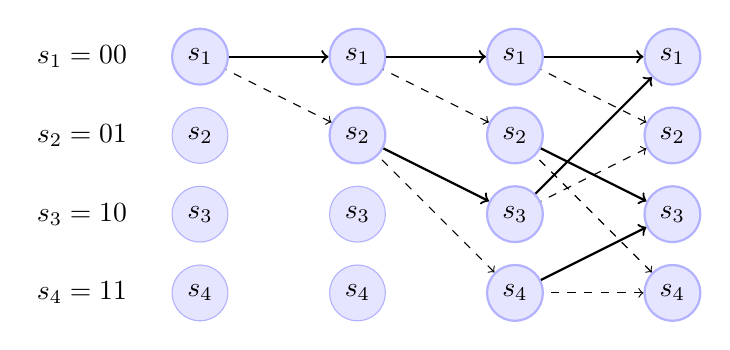
\begin{tikzpicture}[]
% 1st column
\node               at (-1.5,5) {$s_1=00$};
\node               at (-1.5,4) {$s_2=01$};
\node               at (-1.5,3) {$s_3=10$};
\node               at (-1.5,2) {$s_4=11$};
\node[mainstate] (s1_1) at (0,5) {$s_1$};
\node[state] (s2_1) at (0,4) {$s_2$};
\node[state] (s3_1) at (0,3) {$s_3$};
\node[state] (s4_1) at (0,2) {$s_4$};
%\node at (0,1) {Node1};
% 2nd column
\node[mainstate] (s1_2) at (2,5) {$s_1$}
    edge[mainedge] (s1_1);
\node[mainstate] (s2_2) at (2,4) {$s_2$}
     edge[lightedge] (s1_1);

\node[state] (s3_2) at (2,3) {$s_3$};

\node[state] (s4_2) at (2,2) {$s_4$};

%\node at (2,1) {Node2};
% 3rd column
%\node               at (4,6) {$t=2$};
\node[mainstate] (s1_3) at (4,5) {$s_1$}
    edge[mainedge]  (s1_2);

\node[mainstate] (s2_3) at (4,4) {$s_2$}
    edge[lightedge] (s1_2);

\node[mainstate] (s3_3) at (4,3) {$s_3$}
    edge[mainedge] (s2_2);    
\node[mainstate] (s4_3) at (4,2) {$s_4$}
    edge[lightedge] (s2_2);
%\node at (4,1) {Node3};
% 4th column
%\node               at (6,6) {$t=3$};
\node[mainstate] (s1_4) at (6,5) {$s_1$}
    edge[mainedge]  (s1_3)
    edge[mainedge]  (s3_3);
\node[mainstate] (s2_4) at (6,4) {$s_2$}
    edge[lightedge] (s1_3)
    edge[lightedge] (s3_3);
\node[mainstate] (s3_4) at (6,3) {$s_3$}
    edge[mainedge] (s2_3)
    edge[mainedge] (s4_3);
\node[mainstate] (s4_4) at (6,2) {$s_4$}
    edge[lightedge] (s2_3)
    edge[lightedge] (s4_3);
%\node at (6,1) {Node4};

\end{tikzpicture}
	\end{center}
	\caption{MLSE decoding for $\mathcal{A}=\{0,1\}$ and $L=2$. Each state $s_1 ... \; s_4$ represents a possible
	$\mathbf{x}_{\mathrm{i-L+1}}$.}
	\label{fig:trellis}
\end{figure}


For finite state, causal channels, MLSE reduces to the Viterbi Algorithm over a trellis of states.
\\

    \noindent\rule[16pt]{\textwidth}{0.6pt}
	Viterbi Algorithm: (TODO: Decide if this is clear enough)

    \noindent\rule[10pt]{\textwidth}{0.4pt}
    {\footnotesize
    \begin{tabbing}
        {\bf given} $p(y_{\mathrm{i}}|x_{\mathrm{i-L+1}}^{\mathrm{i}}) \; \forall  \;i \in {1..N}$. \\*[\smallskipamount]
        {\bf for $i = 1...N $} \\
         \qquad \= {\bf for each state $s \in \mathcal{A}_{\mathrm{i-L+1}}^{\mathrm{i}}$}\\
        \qquad \qquad \= 1.\ Let $\text{cost}_{s}^{\text{i}} = -\text{log}(p(y_{\mathrm{i}}|x_{\mathrm{i-L+1}}^{\mathrm{i}})) + \underset{s}{\text{min}} \{\text{incoming costs}_{s}^{\text{i-1}}\}$ \\
%        \> 2.\ {\bf break if} $f(z) \leq \hat{f}_{\lambda}(z, x^{k})$. \\
%        \> 3.\ Update $\lambda := \beta \lambda$. \\*[\smallskipamount]
        {\bf return} detected transmission $\hat{\mathbf{x}}$ corresponding to trellis path of $\underset{s}{\text{argmin}} \; \text{cost}_{s}^N $
    \end{tabbing}}
    \noindent\rule[10pt]{\textwidth}{0.4pt}


Note that the Viterbi algorithm is \emph{exponentially} complex in the number of channel states $|\mathcal{A}_{\mathrm{i-L+1}}^{\mathrm{i}}|$, but \emph{linearly} complex in the length of the transmitted sequence $\mathbf{x}$ ($N$ in the algorithm above). 


\subsection{ViterbiNet}
Despite the reduction in MLSE complexity using the Viterbi Algorithm, the metrics $p(y_{\mathrm{i}}|\mathbf{x}_{\mathrm{i-L+1}}^{\mathrm{i}}) ,$ used in each step of the algorithm,
 require knowledge of the channel probability distribution. This may be difficult or costly to obtain. By decomposing with Bayes' theorem, we can instead estimate the individual terms of
\begin{equation*}
p(y_{\mathrm{i}}|\mathbf{x}_{\mathrm{i-L+1}}^{\mathrm{i}}) = 
\frac
{p(\mathbf{x}_{\mathrm{i-L+1}}^{\mathrm{i}}|y_{\mathrm{i}})p(y_{\mathrm{i}})}
{p(\mathbf{x}_{\mathrm{i-L+1}}^{\mathrm{i}})}.
\end{equation*}

\begin{itemize}
\item $p(\mathbf{x}_{\mathrm{i-L+1}}^{\mathrm{i}}|y_{\mathrm{i}})$
: The probability of being in channel state $\mathbf{x}_{\mathrm{i-L+1}}^{\mathrm{i}}$ given the corresponding received symbol $y_{\mathrm{i}}$. If the number of states is finite, the probability mass function over $\mathbf{x}_{\mathrm{i-L+1}}^{\mathrm{i}} \in
|\mathcal{A}_{\mathrm{i-L+1}}^{\mathrm{i}}|$ can be estimated using a neural network for classification as in Figure \ref{nn}. 
	\begin{figure}[H]
	\centering
		\begin{neuralnetwork}[height=4, nodespacing=10mm, layerspacing=15mm]
		\newcommand{\x}[2]{$y_#2$}
		\newcommand{\y}[2]{$s_#2$}
		\newcommand{\hfirst}[2]{\small $h^{(1)}_#2$}
		\newcommand{\hsecond}[2]{\small $h^{(2)}_#2$}
		\newcommand{\hthird}[2]{\small $h^{(3)}_#2$}
		\newcommand{\hfourth}[2]{\small $h^{(4)}_#2$}
		\inputlayer[count=1, bias=false, title=Received\\, text=\x]
		\hiddenlayer[count=2, bias=false, title=\\, text=\hthird] \linklayers
		\hiddenlayer[count=3, bias=false, title=\\, text=\hfourth] \linklayers
		\outputlayer[count=4, title=States\\, text=\y] \linklayers
	    \end{neuralnetwork}
	    	  	  \caption{State classification Neural Network.}
\label{nn}
	\end{figure}

\item $p(y_{\mathrm{i}}) = \sum_{s \in \textit{$\mathcal{S}$}}p(s,y_{\mathrm{i}})$
: The joint probability of channel state $s$ and received signal $y_{\mathrm{i}}$ marginalized over all channel states $\mathcal{S}$. For the case of the LTI channel above, each state $s$ corresponds to a possible symbol sequence $\mathbf{x}_{\mathrm{i-L+1}}^{\mathrm{i}}$. This probability distribution function can be estimated using a mixture-model (Figure \ref{fig:mm}) based on a model for channel noise and training data of received signals (in this case the same data used to train the neural network). The Expectation Maximization Algorithm \cite{ng2000cs229} is used with a chosen model for the channel states and noise. In the case of Gaussian noise, as used here, each state is modeled as a Gaussians. As $p(y_{\mathrm{i}})$ is constant over all states in a given step of the Viterbi algorithm, it may be interpreted as a weighting factor for the cost of a received symbol relative to other symbols in the path. (TODO: More detail on this or enough?)
%\\
%
%    \noindent\rule[16pt]{\textwidth}{0.6pt}
%	Expectation Maximization Algorithm for Gaussian Mixture Model: (TODO Discuss how much derivation is needed here)
%
%    \noindent\rule[10pt]{\textwidth}{0.4pt}
%    {\footnotesize
%    \begin{tabbing}
%        {\bf given} $p(y_{\mathrm{i}}|x_{\mathrm{i-L+1}}^{\mathrm{i}}) \; \forall i \in {1..N}$ . \\*[\smallskipamount]
%        {\bf for $i = 1..N $} \\
%         \qquad \= {\bf for each state $s$ at time $i$}\\
%        \qquad \qquad \= 1.\ Let $\textit{survivor cost}_{s}  += \text{min}\{\text{incoming transition costs}\}$ \\
%%        \> 2.\ {\bf break if} $f(z) \leq \hat{f}_{\lambda}(z, x^{k})$. \\
%%        \> 3.\ Update $\lambda := \beta \lambda$. \\*[\smallskipamount]
%        {\bf return} Symbols corresponding to path of $\underset{s}{\text{argmin}} \; \textit{survivor cost}_{s} $
%    \end{tabbing}}
%    \noindent\rule[10pt]{\textwidth}{0.4pt}


%picture of MM
%	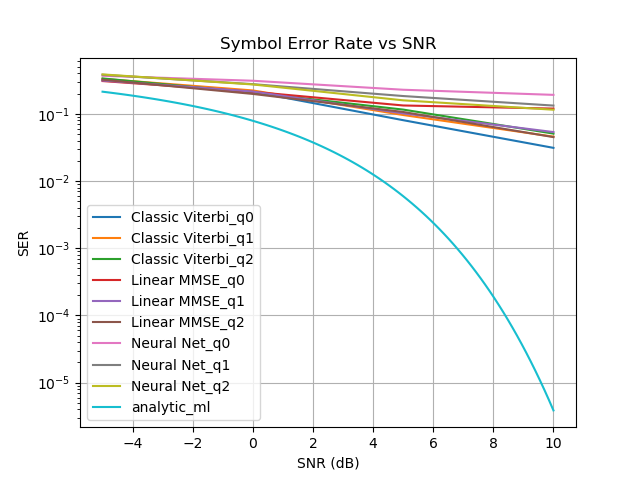
\includegraphics[width=\textwidth,height = 7cm]{results/quant_standard}

\begin{figure}[H]
\centering
	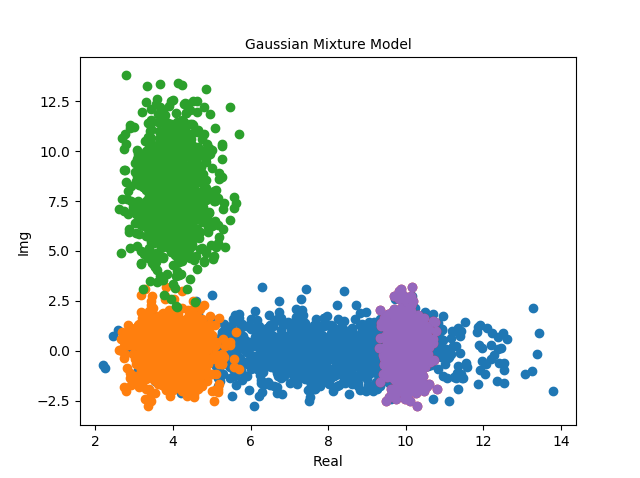
\includegraphics[width=\textwidth,height = 10cm]{system_model/mm}
	  	  \caption{A mixture of complex, Gaussian sources that can be estimate using the Expectation Maximization algorithm}
	  \label{fig:mm}
\end{figure}

\item $p(\mathbf{x}_{\mathrm{i-L+1}}^{\mathrm{i}})$
: The probability of a given transmitted sequence can be neglected for equiprobable transmit symbols.

\end{itemize}

In summary, the metrics $p(y_{\mathrm{i}}|\mathbf{x}_{\mathrm{i-L+1}}^{\mathrm{i}})$ required by the Viterbi algorithm can be estimated using a neural network and a mixture model.






\subsection{A Reduced State ViterbiNet}
While the Viterbi Algorithm complexity scales exponentially in the number of states possible in each step of the algorithm, in some cases this complexity can be reduced without significant degradation of performance. In particular, if the system is such that some states are redundant, these can be combined. The following, relevant example with state redundancy is posed and one potential method of reducing the number of states is considered. 

Consider a received signal
\begin{equation*}
y[k] = \sum_{\mathrm{l=1}}^{\mathrm{L}} a[l]x[k-l] + n[k], \; n[k]  \sim \mathcal{N}(0,1)
\end{equation*}

with $x[k-l] \in \{ -1, +1\}$ and $n[k]  \sim \mathcal{N}(0,1)$.  

In the case of a causal, LTI system with inter-symbol-interference characterized by $\mathbf{a} = [a[1]...a[5]]=[1, 0, .2, .2, .4]$ ($\|\mathbf{a}\|^2_2 = 1$), the received signal (Fig.\ref{fig:redundant_channel}) has fewer than the potential $|\mathcal{A}_{\mathrm{i-L+1}}^{\mathrm{i}}| =2^5$ states as defined above. As one of the channel taps is 0, this will have no impact and thus 16 of the potential 32 states are removed. Further, as there are two taps of value 0.2, these together represent only 3 states rather than 4. 

%\begin{figure}[H]
%\centering
%	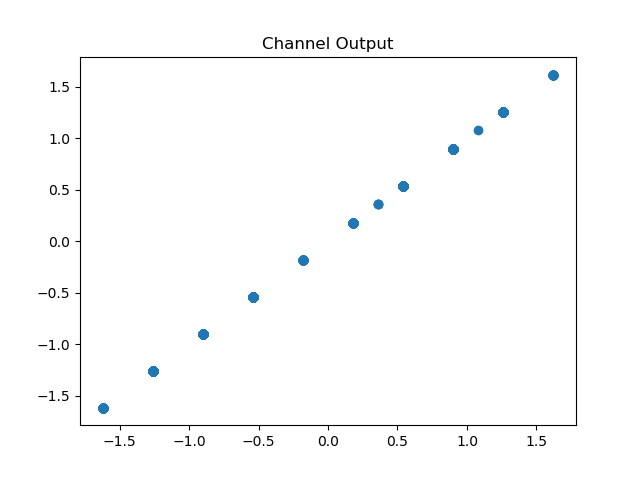
\includegraphics[width=10cm,height = 10cm]{system_model/channel_output}
%	  \label{fig:redundant_channel}
%	  	  \caption{LTI channel with state redundancy with high SNR}
%\end{figure}

One way to exploit state redundancy is to cluster the original states $|\mathcal{A}_{\mathrm{i-L+1}}^{\mathrm{i}}|$  states into a set of $k$ clusters using training data. The K-Means algorithm is proposed as one such method.
\\

    \noindent\rule[16pt]{\textwidth}{0.6pt}
K-Means Clustering Algorithm: A method for unsupervised classification

    \noindent\rule[10pt]{\textwidth}{0.4pt}
    {\footnotesize
    \begin{tabbing}
    {\bf given} initial location $L_c, \forall \;c  \in \{1..K\}$ of K centroids.\\
        {\textbf{for} Number of Iterations}.\\
         \qquad \= {\bf for each training data point $x_{\mathrm{i}}, \;\mathrm{i}  \in \{1..N\}$}\\
        \qquad \qquad \= 1.\ Label $x_i$ with the index c of the closest centroid using $\|x_{\mathrm{i}}- \text{L}_c\|^2_2$. \\
        \qquad \= {\bf for centroid $L_c, \forall \;c  \in \{1..K\}$}\\
                \qquad \qquad \= 1.\ Move $L_{\mathrm{c}}$ to the average location of all training points with label .c\\


%        \> 2.\ {\bf break if} $f(z) \leq \hat{f}_{\lambda}(z, x^{k})$. \\
%        \> 3.\ Update $\lambda := \beta \lambda$. \\*[\smallskipamount]
        {\bf return} Centroid locations.
    \end{tabbing}}
    \noindent\rule[10pt]{\textwidth}{0.4pt}
    
Choosing an appropriate number of clusters will influence the performance of the resulting decoder (Have figure showing this).
\par An implementation point to note is that after clustering the training data into K states, the number of states must be increased to $(|\mathcal{A}_{\mathrm{i}}|)\text{K}$. In the above example 2K. The Viterbi algorithm selects a symbol sequence corresponding to a path of state transitions through the trellis. In order to make the correspondence between a unique path and a symbol sequence, each state transition must represent a transmitted symbol. \emph{Each} resulting centroid from the k-means clustering is associated to \emph{each} potential transmit symbol in order to create a "shorter" trellis for which each state transition still represents a transmitted symbol. 

(TODO:Discuss minimum phase representations for channels and why this might be an advantage?)


\section{Results}
\subsection{A supervised equalization benchmark}
The Linear Minimum Mean-Squared Error (LMMSE) equalizer derived below is used provide a linear equalization reference to the non-linearity of the proposed neural network, mixture model equalization.
\par
Given an estimate of channel memory length L, the convex and continuously differentiable optimization problem 

\begin{equation*}\label{mmse}
\underset{\mathbf{\mathbf{h}} \in \textit{$\mathcal{C}^{\text{L}}$}}{\text{argmin}} \;
 E[\|x-\mathbf{h}^T\mathbf{y}\|^2],
\end{equation*}\
minimizes the squared error of the linearly detected symbol $\mathbf{h}^T\mathbf{y}$ and true symbol $x$.
Using
\begin{equation*}\label{mmse}
\frac{\partial  E[\|x-\mathbf{h}^T\mathbf{y}\|^2]}{\partial \mathbf{h} } = 0
\end{equation*}
the optimal LMMSE equalizer is \cite{proakis1988introduction}
\begin{equation*}\label{mmse}
\mathbf{h} = E[\mathbf{R}_{yy}]^{-1}E[\mathbf{r}_{yx}].
\end{equation*}
$E[\mathbf{R}_{yy}]$ and $E[\mathbf{r}_{yx}]$ are estimated by
\begin{equation*}\label{mmse}
 E[\mathbf{R}_{yy}]= \frac{1}{\mathrm{N}}\sum_{\mathrm{i=1}}^{\mathrm{N}}
\mathbf{y^{\text{i}}_{\text{i-L+1}}}\mathbf{y^{\text{i}}_{\text{i-L+1}}}^H
 \end{equation*}
 and
\begin{equation*}\label{mmse}
E[\mathbf{r}_{yx}]= \frac{1}{\mathrm{N}}\sum_{\mathrm{i=1}}^{\mathrm{N}}
\mathbf{y^{\text{i}}_{\text{i-L+1}}}x_{\text{i}}
;
 \end{equation*}
 using the same training data as the neural network and mixture model. 


\subsection{Simulation Details}
\subsubsection{System Model}
Verification and further testing of the implementation and integration of the algorithms described above is performed using the following system model.

%\begin{tikzpicture}[node distance=2cm]
%\node (start) [process] {Symbol Stream};
%\node (channel) [process, right = of start] {Channel};
%\draw [arrow] (start) -- (channel);
%
%\end{tikzpicture}

\begin{equation*}
y[\text{k}] = f_{\text{k}}(\mathbf{x}) + n[\text{k}].
\end{equation*}
With $x[\text{k}] \in \{ -1, +1\}$, independent $n[\text{k}]\sim \mathcal{N}(0,1)$ and 
\begin{equation*}
\text{SNR} = \frac{E\{|x[\text{k}]|^2\}}{\sigma^2}.
\end{equation*}

Note that each received signal $y[\text{k}] $ is potentially a function of all input symbols (assume causality?). Decoding performance for different values of the channel function $f_{\text{k}}()$ are evaluated. 

\subsubsection{Algorithm Parameters}
The parameters for the algorithms used in this work are detailed below.
\begin{itemize}
\item \textbf{Neural Network}
\begin{itemize}
\item Architecture: 4 layers {1, 100 (Tanh activation), 50 (relu activation), $M^L$ (Softmax $\rightarrow$ Negative Log-Likelihood)}
\item Training Data Examples: 5000
\item Neural Network Updates: Admm \cite{kingma2014adam} with step size $10^{-2}$ 
\item Batch Size: 1000 
\item Backpropogation Updates (Epochs): 900
\item Loss Function: Cross Entropy
\end{itemize}
\item \textbf{Expectation Maximization Algorithm}
\begin{itemize}
\item Training Data Examples: 5000
\item Mixture Model Source Types: Gaussian
\item Number of Sources: Number of channel states
\end{itemize}
\item \textbf{K-Means Algorithm (For Reduced State ViterbiNet)}
\begin{itemize}
\item Training Data Examples: 5000
\end{itemize}
\end{itemize}


\subsection{Simulation Results}
We first evaluate the detector performance using the Linear Time Invariant channel

\begin{equation*}
y[\text{k}] = \sum_{\mathrm{l=1}}^{\mathrm{L}} a[l]x[\text{k}-l] + n[\text{k}].
\end{equation*}
with impulse response $a[l] = ...$.
Simulation results are shown in fig \ref{fig:LTI performance}
\begin{figure}[H]
	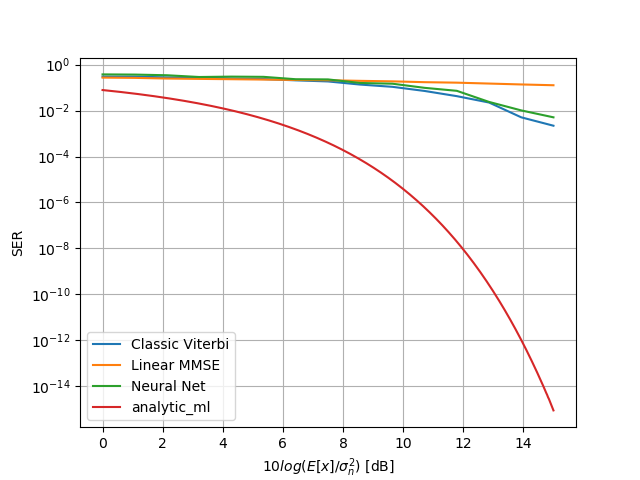
\includegraphics[width=\textwidth,height = 10cm]{results/lti_normal}
		  \caption{Detection performance over LTI channel with AWGN}
	  \label{fig:LTI performance}
\end{figure}

\subsubsection{LTI + Quantizer Channel}

To evaluate decoder performance in the non-linear channel setting, we apply a quantizer, $Q()$, to the output of the previous LTI + AWGN channel.
\begin{equation*}
y[\text{k}] = Q(\sum_{\mathrm{l=1}}^{\mathrm{L}} a[l]x[\text{k}-l]) + n[\text{k}].
\end{equation*}
 Here we evaluate performance under two levels of quantization severity: rounding channel output down to a given number of decimal places . Figure \ref{fig:Quantized Overlay} depicts the quantizer and its impact on the received symbols from the LTI channel. The resulting performance is seen in Figure \ref{fig:Quantized performance}. Notice that this is essentially a reduction of the original channel states as there is now redundancy that was not previously present. 

\begin{figure}[H]
\centering
	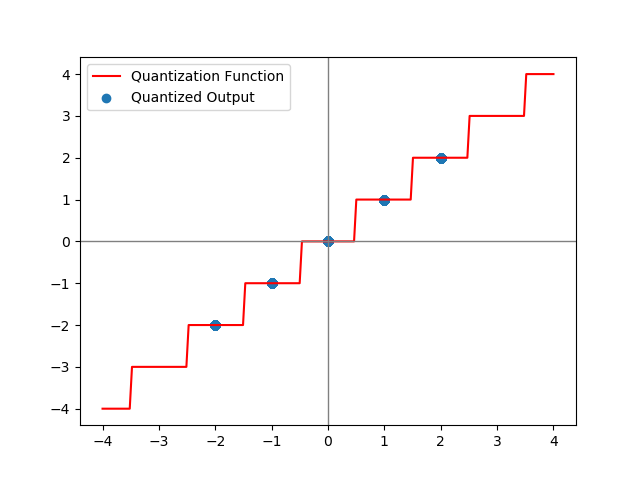
\includegraphics[width=10cm,height = 10cm]{system_model/quantizer_overlay}
			  \caption{Quantized output of LTI channel overlayed on the applied quantization function. TODO decide on axis titles }
	  \label{fig:Quantized Overlay}
\end{figure}

\begin{figure}[H]
	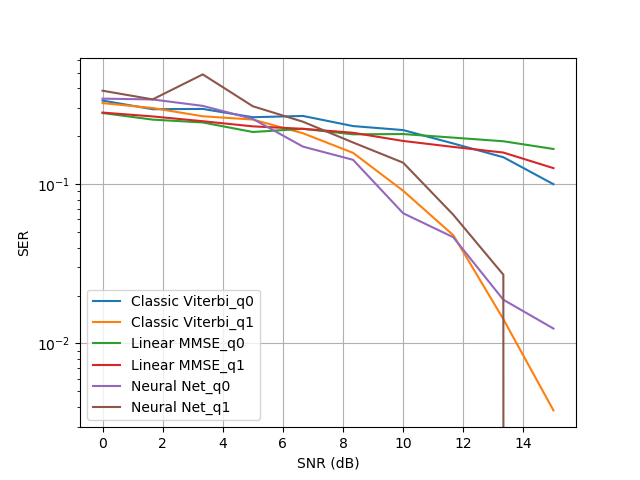
\includegraphics[width=\textwidth,height = 10cm]{results/quantized_before_noise}
		  \caption{Detection performance over LTI channel with AWGN and quantization}
	  \label{fig:Quantized performance}
\end{figure}


\subsubsection{molecular communication Channel}
Lastly, the performance of the neural network based detector is evaluated data collected from a molecular communication channel. ... Explain if there are any results to report. 

\section{Conclusion}
The proposed detection method from \cite{shlezinger2019viterbinet} is evaluated in channels for which $p(y_{\mathrm{i}}|\mathbf{x}_{\mathrm{i-L+1}}^{\mathrm{i}}),$ is unknown and non-linear. Simulation results indicate that this detector can successfully learn
$p(y_{\mathrm{i}}|\mathbf{x}_{\mathrm{i-L+1}}^{\mathrm{i}})$ for non-linear channels. A method for reducing the complexity of the resulting Viterbi Algorithm is also proposed, however the method of state reduction for the channel needs to be further investigated to improve the poor performance observed. 
\par 
In this work the MLSE is found using the Viterbi Algorithm. The same metrics can also be used in optimizing other performance metrics. In \cite{shlezinger2020datadriven} these estimate metrics have been used for minimize bit error rate estimation using the BCJR algorithm. 

Extensions of specific work: 
More on reduced state.
Using other channels and repeat online type of updates for dynamic channels for these more challenging channels. 
Learning channel changes in cases for which coherence time is shorter than updates to network made by pilot symbols. 

General method extensions:


\newpage
\bibliography{report_bib}{}
\bibliographystyle{plain}
\end{document}
